% The reach of the construction --- plan \S4.6.  Merges draft \S6 (spectrum)
% and \S7 (HIV), compressed from 5217 words.
% Sources: new_notes3 Part F \S26--\S29, Part G \S30--\S32; new_notes2 \S11
% (Hataye findings, stage equations), \S12 (reset), \S13 (linear vs
% exponential growth), \S14 (Cases 1--5), \S15 (self-excitation), \S16
% (partial release).  The menus of \S6.3--\S6.4 are in Appendix E.

\section{The reach of the construction}
\label{p:sec:reach}

\Cref{p:sec:generality} showed that any pair of kernels induces the same
population equations. Bursting and constant budding are the ends of a
spectrum (\cref{p:fig:spectrum}); between them lie mechanisms that release
many times per cell, release part of the load, or release in a self-excited
cascade, and beyond it lie multi-stage models that are not
birth--death--catastrophe processes at all. All supply a pair $(S,g)$, and
none changes \cref{p:eq:skeleton}. The section closes on where that
generality stops.

\begin{figure}[tbp]
\centering
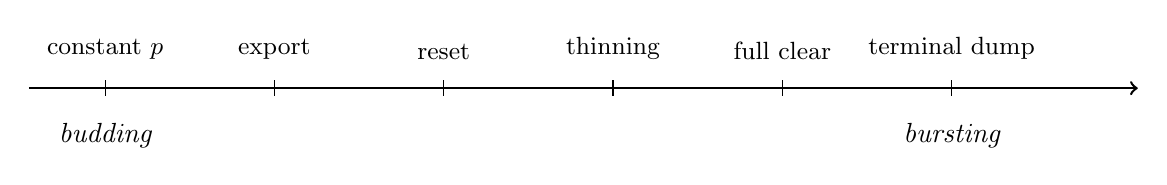
\begin{tikzpicture}[x=2.15cm,y=0.70cm,font=\small]
\draw[->,line width=0.9pt] (0,0) -- (6.55,0);
\foreach \x in {0.45,1.45,2.45,3.45,4.45,5.45}
  \draw (\x,-0.14) -- (\x,0.14);
\node[above=7pt] at (0.45,0) {constant $p$};
\node[above=7pt] at (1.45,0) {export};
\node[above=7pt] at (2.45,0) {reset};
\node[above=7pt] at (3.45,0) {thinning};
\node[above=7pt] at (4.45,0) {full clear};
\node[above=7pt] at (5.45,0) {terminal dump};
\node[below=9pt,font=\itshape] at (0.45,0) {budding};
\node[below=9pt,font=\itshape] at (5.45,0) {bursting};
\end{tikzpicture}
\caption{The budding--bursting spectrum. Every station is a choice of
$(S,g)$.}
\label{p:fig:spectrum}
\end{figure}

\subsection{A finite-dimensional shadow: five ODE cases}
\label{p:sec:odecases}

When a fitting-ready ODE is wanted rather than a convolution, the same ideas
assemble into a ladder of five cases (\cref{p:tab:cases}), written out in
\cref{p:app:catalogue}. Classical BMVR is Case~1
(\cref{p:eq:case1}); stock-and-export recovers it in the fast-export limit
(\cref{p:eq:case3qss}); load-proportional dumps are Cases~4--5
(\cref{p:eq:case4,p:eq:case5R0}). Each case also induces kernels, so
\cref{p:eq:skeleton} stays available whenever stage structure is traded for
age structure.

\begin{table}[htbp]
\centering
\renewcommand{\arraystretch}{1.12}
\small
\begin{tabular}{@{}p{0.30\textwidth}p{0.34\textwidth}p{0.22\textwidth}@{}}
\toprule
Case & Intracellular story & Free-particle source \\
\midrule
1 Classic & none (instant release) & $p\,\Icell$ \\
2 Eclipse $+$ classic & delay $E\to\Icell$, then as 1 & $p\,\Icell$ \\
3 Stock $+$ continuous export & $\nu$ into $Q$, export $\varepsilon Q$ & $\varepsilon\,Q$ \\
4 Stock $+$ full clear & $\nu$ into $Q$, dump $\propto Q^2/\Icell$ & $\delta Q^2/\Icell$ \\
5 Eclipse $+$ stock $+$ full clear & $E\to\Icell$, then as 4 & $\delta Q^2/\Icell$ \\
\bottomrule
\end{tabular}
\caption{The five ODE cases. Case~5 is Case~4 composed with Case~2's
eclipse block; the ladder is ordered by how load-dependent the release
term is.}
\label{p:tab:cases}
\end{table}

\subsection{Reset catastrophe: the worked intermediate}
\label{p:sec:reset}

The absorbing process releases at most once per cell. The intermediate
worth isolating lets a cell release \emph{many} times: while the cell is
alive the load undergoes birth $\lambda n$, death $\mu n$, optional
immigration $\nu$, and a \emph{dump that resets} --- at rate $\delta n$ the
whole pool is released and the load returns to zero, after which it may
re-accumulate --- with the cell dying at a separate, load-independent rate
$d_{\Icell}$. Reading the load as a local assembled pool rather than the
whole-cell contents makes this a tractable multi-pulse caricature between
full dumping and many small exports.

Because dumps do not absorb, the kernels change but the skeleton does not:
\begin{equation}
S(\alpha)=\ee^{-d_{\Icell}\alpha},
\qquad
g(\alpha)=\delta\,\ee^{-d_{\Icell}\alpha}\,\mean{X_\alpha^2},
\label{p:eq:reset-kernels}
\end{equation}
where $\mean{X_\alpha^2}$ is computed for the non-absorbing reset process.
Linear rates keep its moments tractable, so $g$ is explicit once they are
solved, and structurally $g\propto\mean{X^2}$ exactly as for the absorbing
process. The renewal system is identical in form to
\crefrange{p:eq:Icell}{p:eq:Vfree}, with
\begin{equation}
p_{\rm eff}(r)=\lrb{r+d_{\Icell}}\Lap{g}(r),
\qquad
d_{\Icell,{\rm eff}}\equiv d_{\Icell},
\label{p:eq:reset-peff}
\end{equation}
and $R_0=(\gamma T/c)\int_0^\infty g$, finite only for $d_{\Icell}>0$, since
otherwise recurrent dumps could continue forever. If the reset process
admits a stationary law $\pi$ and $d_{\Icell}$ is small, the mature-cell
limit is
\begin{equation}
p_\infty=\lim_{\alpha\to\infty}\frac{g(\alpha)}{S(\alpha)}
=\delta\,\mathbb{E}_\pi[X^2]:
\label{p:eq:reset-mature}
\end{equation}
a long-lived infected cell behaves as classical constant-$p$ BMVR with that
$p$, while transients --- first dumps, young cells --- still need the full
kernel. An eclipse is added as before: set $g(\alpha)=0$ for $\alpha<\tau_e$
and keep $S$. This is what makes the spectrum claim concrete rather than
gestural (\cref{p:tab:reset}): an intermediate with kernels, an effective
release rate, a mature limit, and a definite answer as to which classical
model it converges on.

\begin{table}[htbp]
\centering
\renewcommand{\arraystretch}{1.1}
\small
\begin{tabular}{@{}lll@{}}
\toprule
 & Absorbing BDC & Reset catastrophe \\
\midrule
After dump & process ends in $H$ & $X\to0$, continues \\
Dumps per cell & $\le1$ & many, until cell death \\
Survival kernel & $\Ifix$ & $\ee^{-d_{\Icell}\alpha}$ \\
Release kernel & $\delta K_{\rm BDC}(\alpha)$ & $\delta \ee^{-d_{\Icell}\alpha}\mean{X_\alpha^2}$ \\
Population equations & renewal BMVR & same form \\
Mature limit & not constant budding & $p\to\delta\,\mathbb{E}_\pi[X^2]$ \\
\bottomrule
\end{tabular}
\caption{Absorbing against resetting catastrophe. Only the kernels differ;
the population layer does not know which it has been given.}
\label{p:tab:reset}
\end{table}

\subsection{Partial release}
\label{p:sec:partial}

The last axis is \emph{how much} leaves the cell when a release event
fires. Cases~3--5 sit at the extremes, continuous export and full clear; the
natural intermediate removes a random part of the load. Two ingredients are
free: the event clock $\lambda(X)$ --- constant $\delta$, linear $\delta X$,
or cooperative $\delta X^2$ --- and the law of the amount released. The
default is boolean thinning, each unit released independently with
probability $\varphi$; the other options are catalogued in
\cref{p:app:catalogue}. One result organises the axis. At the mean-field level with $\lambda=\delta
X$, the population equations are Case~4 scaled by $\varphi$:
\begin{equation}
\ddt{\Icell}=\gamma T\,\Vfree-d_{\Icell}\Icell,
\qquad
\ddt{Q}=\nu\Icell-\delta\varphi\,\frac{Q^2}{\Icell}-d_{\Icell}Q,
\qquad
\ddt{\Vfree}=\delta\varphi\,\frac{Q^2}{\Icell}-c\,\Vfree.
\label{p:eq:partial}
\end{equation}
With a constant clock $\lambda=\delta$ instead, the mean export is
$\delta\varphi Q$ and the bulk equations collapse to Case~3 with
$\varepsilon_{\rm eff}=\delta\varphi$. So partial release is invisible in
the mean-field equations whenever the event clock is load-independent, and
visible when it is load-dependent; in single-cell release-count
distributions it is always visible. Where in $\varphi$ the flooding advantage
of \cref{p:thm:flood} survives is open, and the closed-form structure may not
persist at intermediate $\varphi$ at all.

\subsection{Self-exciting release}
\label{p:sec:selfexcite}

Release may also be partially \emph{self-exciting}: one event makes further
release more likely for a short time, through cooperative nucleation, local
membrane platforms, or machinery already recruited at a site. Open-ended
self-excitation is implausible, since stock depletes and machinery is
finite, but the skeleton accommodates any hybrid of excitation, refill and
depletion, because a renewal model exists whenever
$g(\alpha)=\mean{\lambda(\alpha)\mid\text{alive}}$ is computable. A finite
ODE model needs the excitation carried by a low-dimensional Markov state.
The exponential-kernel Hawkes process \cite{hawkes1971spectra} is the case
in which it is: Markovian in a shot-noise intensity, and so
ODE-representable. The general event-history form is not.
\Cref{p:app:catalogue} catalogues twelve candidates and develops four.

\subsection{A non-BDC instance: HIV}
\label{p:sec:hiv}

This chapter's results are written for pathogens whose intracellular life
ends in load-proportional catastrophe. HIV is not one: it buds from the
plasma membrane, and an infected cell need not rupture in one event. Yet
single-cell and limiting-dilution data show something surge-like --- long
quiet periods, then a concentrated bout of release --- which is the
phenomenon the birth--death--catastrophe process exists to explain. The position
taken here is neither to force HIV into that process nor to retreat to
constant-$p$ BMVR, but to build an eclipse-structured,
short-productive-pulse model on the same skeleton.

Hataye et al.\ \cite{hataye2019principles} coupled limiting-dilution
latency-reactivation cultures to stochastic models. The cultures show delay
plus a short pulse, not a terminal dump: first detection around day~3, bulk
production over days~3--5, an Erlang eclipse with $n\approx5$, and many
silent lineages ($f_{\rm HIV}\approx0.41$). Establishment against the number
of virus-releasing cells is sigmoid, which they read as an Allee effect,
with threshold $\Lambda\approx2.3$ cells (about $5100$ RNA copies under a
$\ge2\times10^5$ definition) and about $2\%$ establishment from one
stimulated cell. Those numbers are collected in \cref{p:tab:hataye};
\cref{p:tab:hiv-support,p:tab:hiv-contrast} record what they support and
what they do not.
% NEEDS-REF: Allee effects and stochastic establishment theory

\begin{table}[htbp]
\centering
\renewcommand{\arraystretch}{1.12}
\small
\begin{tabular}{@{}p{0.46\textwidth}p{0.46\textwidth}@{}}
\toprule
Supported for HIV & Not supported as literal HIV \\
\midrule
Multi-stage eclipse (delay) & Pure one-type BDC terminal catastrophe \\
Short productive pulse then cell death & Memoryless constant-$p$ BMVR from $t=0$ \\
High stochasticity; many silent lineages & Independent branching alone near threshold \\
Renewal / stage structure for free virus & QSD $=$ geometric burst size as an HIV law \\
Allee / synergistic establishment & \\
\bottomrule
\end{tabular}
\caption{What the limiting-dilution data support, and what they do not.
The right-hand column is the list of claims this chapter does not make for
HIV.}
\label{p:tab:hiv-support}
\end{table}

\begin{table}[htbp]
\centering
\renewcommand{\arraystretch}{1.1}
\small
\begin{tabular}{@{}lll@{}}
\toprule
 & Lytic BDC (this chapter) & HIV (Hataye-guided) \\
\midrule
Release mechanism & catastrophe at rate $\delta X$ & budding while productive \\
End of production & terminal; process absorbed & short productive life; cell dies \\
Intracellular load $X$ & explicit birth--death state & not required as primary state \\
Quiet period & until first catastrophe & multi-stage eclipse ($+$ latency) \\
Sustained multi-day release & one large dump (or nothing) & often staggered short pulses \\
Establishment theory & independent offspring as baseline & Allee synergy near threshold \\
Natural hosts & \yp{}, \ft{}, phage & CD4 T-cell latency / rebound \\
\bottomrule
\end{tabular}
\caption{Two mechanisms, compared where they differ. The seam is the
release event: terminal and load-proportional on the left, repeated and
load-independent on the right.}
\label{p:tab:hiv-contrast}
\end{table}

\paragraph{Candidate stage structure.} What the data ask for is a two-path
eclipse feeding a short productive class, drawn in \cref{p:fig:hiv-stages}:
a stimulated latent cell $L_0$ enters either a multi-stage path $A$ of high
release potential or a brief path $B$ of low potential, eclipse cells divide
or die without releasing, and productive cells release at constant rate
until they die. The reaction list and the stage equations it induces are
\cref{p:app:hivstages}; only two features matter here. The delay comes from
the length of the chain rather than from any slow release rate, and eclipse
proliferation is a genuine source term rather than a relabelling --- which
is what lets a single reactivated lineage produce multi-day detection
without any one cell budding for days.

\begin{figure}[tbp]
\centering
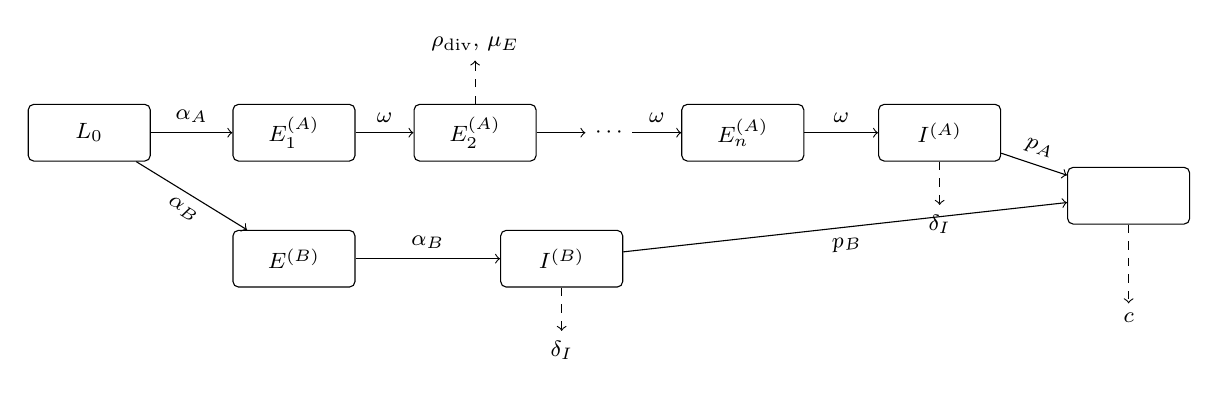
\begin{tikzpicture}[font=\footnotesize,
  box/.style={draw,rounded corners=2pt,minimum height=0.72cm,
              minimum width=1.55cm,align=center}]
% pathway A (upper)
\node[box] (L0)  at (0,1.6) {$L_0$};
\node[box] (E1)  at (2.6,1.6) {$E_1^{(A)}$};
\node[box] (E2)  at (4.9,1.6) {$E_2^{(A)}$};
\node      (Ed)  at (6.6,1.6) {$\cdots$};
\node[box] (En)  at (8.3,1.6) {$E_n^{(A)}$};
\node[box] (IA)  at (10.8,1.6) {$I^{(A)}$};
% pathway B (lower)
\node[box] (EB)  at (2.6,0) {$E^{(B)}$};
\node[box] (IB)  at (6.0,0) {$I^{(B)}$};
% free virus
\node[box] (V)   at (13.2,0.8) {$\Vfree$};
% arrows
\draw[->] (L0) -- node[above,sloped] {$\alpha_A$} (E1);
\draw[->] (E1) -- node[above] {$\omega$} (E2);
\draw[->] (E2) -- (Ed);
\draw[->] (Ed) -- node[above] {$\omega$} (En);
\draw[->] (En) -- node[above] {$\omega$} (IA);
\draw[->] (L0) -- node[below,sloped] {$\alpha_B$} (EB);
\draw[->] (EB) -- node[above] {$\alpha_B$} (IB);
\draw[->] (IA) -- node[above,sloped] {$p_A$} (V);
\draw[->] (IB) -- node[below,sloped] {$p_B$} (V);
% losses
\draw[->,dashed] (IA.south) -- ++(0,-0.55) node[below] {$\delta_I$};
\draw[->,dashed] (IB.south) -- ++(0,-0.55) node[below] {$\delta_I$};
\draw[->,dashed] (E2.north) -- ++(0,0.55)
  node[above] {$\rho_{\rm div},\,\mu_E$};
\draw[->,dashed] (V.south) -- ++(0,-1.0) node[below] {$c$};
\end{tikzpicture}
\caption{The stage structure of \cref{p:eq:hiv-paths}: two eclipse pathways
from the stimulated latent class $L_0$ --- a multi-stage path $A$ of high
release potential and a brief path $B$ --- each feeding a short productive
class releasing at constant rate. Division and death (dashed) act in
eclipse, death $\delta_I$ in the productive classes, clearance $c$ on free
virus. The source of the delay is the chain, not the release rate.}
\label{p:fig:hiv-stages}
\end{figure}

For ongoing infection the initial cohort becomes incidence, split between
pathways with $\pi_A+\pi_B=1$:
\begin{equation}
i(t)=f\bigl(\Vfree(t),T\bigr),
\qquad
\text{source into }E_1^{(A)}=\pi_A i(t),
\qquad
\text{source into }E^{(B)}=\pi_B i(t).
\label{p:eq:hiv-incidence}
\end{equation}
Linear infection, $f(\Vfree,T)=\gamma T\Vfree$, recovers a stage-structured
BMVR. Near the threshold, though, the data favour a sigmoid law over
independent per-virion success; the minimal upgrade is the Allee incidence
\begin{equation}
f(\Vfree,T)=\gamma T\,\Vfree\cdot\frac{\Vfree}{K_A+\Vfree},
\label{p:eq:allee}
\end{equation}
inefficient at very low $\Vfree$ and saturating to mass action for
$\Vfree\gg K_A$, with $K_A$ set so that cumulative initial release near
$\sim5\times10^3$ RNA copies sits at the inflection of establishment
probability. More mechanistic forms can replace it; the point is that
linearity in $\Vfree$ alone is not faithful near establishment. Writing
$g_{\rm HIV}$ for the expected release rate at age $\alpha$ after a single
infection or reactivation and $S_{\rm HIV}$ for the probability of still
being in a productive lineage, \cref{p:eq:skeleton} holds exactly:
\begin{equation}
\Icell(t)=\Icell_0S_{\rm HIV}(t)+(i*S_{\rm HIV})(t),
\qquad
\ddt{\Vfree}=\Icell_0g_{\rm HIV}(t)+(i*g_{\rm HIV})(t)-c\,\Vfree(t).
\label{p:eq:hiv-renewal}
\end{equation}
Here $g_{\rm HIV}$ is \emph{not} $\delta K$: it is the density of productive
sojourn times, weighted by $p_A$ and $p_B$, with the Erlang eclipse supplying
the delay --- near zero for small $\alpha$, then rising and falling, which is
the mathematical expression of nothing for a long time, then a lot. The
effective parameters carry over under
$(\Ifix,g)\mapsto(S_{\rm HIV},g_{\rm HIV})$:
\begin{equation}
p_{\rm eff}(r)=\frac{\Lap{g}_{\rm HIV}(r)}{\Lap{S}_{\rm HIV}(r)},
\qquad
R_0=\frac{\gamma T}{c}\int_0^\infty g_{\rm HIV}(\alpha)\,\dd\alpha
\quad\text{(linear incidence)},
\label{p:eq:hiv-peff}
\end{equation}
while under \cref{p:eq:allee} $R_0$ remains the large-population threshold
and early establishment is governed in addition by the scale $K_A$.

\paragraph{Linear or exponential intracellular growth.} HIV does not
amplify infectious units by branching: after integration the template count
is one or a few proviruses, and structural products do not self-replicate.
Production is immigration-like: the mean load follows
$\bar x'\approx\nu-\mu\bar x$, set by a fixed template count, rather than
the $\bar x'=r\bar x$ of a process in which each unit begets more units.
That is the whole reason the release kernel cannot be $\delta K$. The regime
adopted here is eclipse then mean-linear accumulation.

\subsection{Where the reach stops}

The skeleton is general; the results proved on it are not. What carries over
to any single-cell mechanism is \cref{p:eq:skeleton}, the map
$p_{\rm eff}=\Lap g/\Lap S$, the reading of constant $p$ as an
exponential-phase projection, and the generation-kernel formulation of $R_0$
and $r$. What does not is everything resting on the closed forms of the
birth--death--catastrophe process: the flooding criterion
$1/\delta<1/\lambda+1/\mu$, the geometric burst law and its identification
with the quasi-stationary distribution, one-shot cumulative release as the
only single-cell trajectory. For HIV, independent branching is not the full
establishment story near the observed threshold; the flooding comparison
survives as a \emph{linear} baseline, at matched mean yield with offspring
variances compared. But near $\sim5\times10^3$ RNA copies synergy can
dominate variance effects, and the two mechanisms must be separated before
either is invoked.

\FloatBarrier
